\section{Part 2 Task 2}

\subsection{Simple Introduction}

In this part, I need sample 25 images from my trained GAN. And I will do this at the start of training, halfway through training and after training has terminated.

\subsection{Default Parameters}

\begin{itemize}
  \item \texttt{n\_epochs}: $200$, maximum number of epochs to train the model
  \item \texttt{batch\_size}: $64$, batch size for training
  \item \texttt{lr}: $0.0002$, learning rate for optimization
  \item \texttt{latent\_dim}: $100$, dimension of input noise
  \item \texttt{save\_interval}: $500$, interval for saving images generated.
\end{itemize}

I use \texttt{torch.optim.Adam()} for optimizer, \texttt{torch.nn.BCELoss()} for loss function.

\subsection{Result Visualization}

Fig \ref{fig:p2t2_train} shows the results of 25 sample images at the start of training, halfway through training and after training has terminated.

\begin{figure}[!htbp]
  \centering
  \begin{subfigure}[b]{0.3\textwidth}
    \includegraphics[width=\textwidth]{img/p2t2/0.png}
    \caption{Start ($0/187,500$)}
  \end{subfigure}
  \begin{subfigure}[b]{0.3\textwidth}
    \includegraphics[width=\textwidth]{img/p2t2/1000.png}
    \caption{Start ($1,000/187,500$)}
  \end{subfigure}
  \begin{subfigure}[b]{0.3\textwidth}
    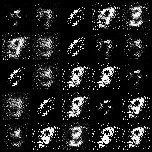
\includegraphics[width=\textwidth]{img/p2t2/10000.png}
    \caption{Start ($10,000/187,500$)}
  \end{subfigure}
  \begin{subfigure}[b]{0.3\textwidth}
    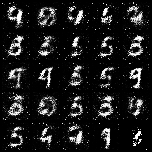
\includegraphics[width=\textwidth]{img/p2t2/20000.png}
    \caption{Middle ($20,000/187,500$)}
  \end{subfigure}
  \begin{subfigure}[b]{0.3\textwidth}
    \includegraphics[width=\textwidth]{img/p2t2/90000.png}
    \caption{Middle ($90,000/187,500$)}
  \end{subfigure}
  \begin{subfigure}[b]{0.3\textwidth}
    \includegraphics[width=\textwidth]{img/p2t2/187500.png}
    \caption{End ($187,500/187,500$)}
  \end{subfigure}
  \caption{Task 2 Training Process}
  \label{fig:p2t2_train}
\end{figure}

\subsection{Result Analysis}

\subsubsection{Overall Analysis}

It can be intuitively seen from the figure that: at the very beginning, the so-called "images" generated are just simple noise points, which have nothing to do with the MNIST handwriting data set

When the training reaches half (approximately $20,000 \sim 90,000$ iterations),
the Generator has been able to generate images that are similar to the handwritten digits data set, but there is some noise and the shape of the handwritten digits is not very stable.

When the training is completely completed (approximately $180,000$ iterations),
compared with the first two, there are fewer noise points, and the shape of the handwritten numbers is more specific and clear, indicating that the result of training is much better.

\subsubsection{Training Analysis}

Observing the output image, we can find that in the initial stage of training, the influence of learning is relatively great.
The noise that was still meaningless at about $10,000$ iterations, had begun to take on a digital shape by $20,000$ iterations.

But comparing $90,000$ and $180,000$, the marginal diminishing effect appears clearly:
compared with the previous training, the gap between them is not very obvious, and even after training for $180000$ iterations, the generation of handwritten data still has not a completely clear part.

\subsubsection{Network Analysis}

One consideration is the structure of my GAN network itself.
In fact, in this assignment, following the suggestions on the template, I used linear layers as the main part of the network.
According to the comparison of Assignment 2, we already know that in problems related to image processing, convolutional layers often has better results than linear layers.
So I think that if I use the convolutional generator structure such as Fig \ref{fig:p2_gan_struct}, I may get better image generation results.
